\chapter[SCP-140 未完编年史]{
    SCP-140 An Incomplete Chronicle\\
    SCP-140 未完编年史
}

\label{chap:SCP-140}

\begin{figure}[H]
    \centering
    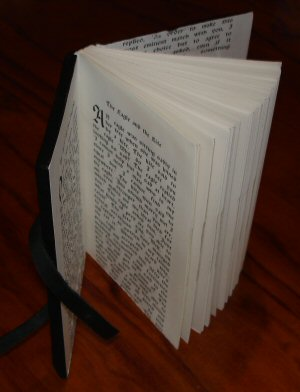
\includegraphics[width=0.5\linewidth]{images/SCP-140.jpg}
    \caption*{一份SCP-140的复制品}
\end{figure}

\bb{项目编号:}SCP-140

\bb{项目等级:}Keter

\bb{特殊收容措施:}SCP-140绝对禁止被置于任何来源的标准墨水,人类血液,或其他可用于书写的液体的15米范围内。任何由血液或墨水造成的污染必须立即上报。所有由最初的印刷所创造的SCP-140的副本必须尽可能找到并加以摧毁。只有SCP-140允许保存——基于研究、预警、索引、和尽可能从其记载中根据文字主题推断出其他SCP 物品。

SCP-140被保存于Site-76一间容纳一个单独书桌的密封金库中。当前没有研究行为实施在最初版本的SCP-140上。研究人员允许阅读不经其作者笔迹而没有异常特性的副本。在研究行为被允许的场合下,不能将SCP-140移离其仓库,阅读者与之接触的时间不能超过█小时。其使用权仅限于明确的研究目的,需要获取首席研究人员的书面批准。一名武装守卫将把守于金库外并对任何偷窃尝试施以致命性攻击。

如果任何人员开始显示出对SCP-140的痴迷或表现出任何可能的模因污染迹象,他们将被进行A 级记忆清除,需要植入伪造记忆并调离至其他项目。被转移人员必须被监视以防复发。

\bb{描述:}SCP-140是一本现代的硬皮书籍,加以不起眼的黑色装桢,有未知数量的白色书页。书的封皮不见了,但是其书名“王朝编年史”清晰可见。其扉页有作者的署名,其姓名无法辨认。文字显示其版权年份为19██年。仔细地检查发现其封皮中所包含的书页数目远比其能容纳的数目要多。

其阅读者承认在阅读SCP-140时出现的妄想,不安,以及偶尔的恶心,虽然这可能和其构成材料有关。虽然如此,读者大都一致描述SCP-140为迷人的并表达了继续阅读的兴趣,尽管它时常出现令人不安的内容。十五分之一的读者描述它有轻微的干掉的血的气味。

SCP-140详细地描述了一个起源于现西伯利亚中南部的文明,确认为“Daevites”。虽然Daevites像所有其他文明一样随着时间流逝逐渐进化和改变,但他们似乎具有某种不同寻常的一致性。通常Daevites文明在所有时期的固定特色包括有尚武,侵略性,先祖崇拜,在城镇中心统治数量巨大的奴隶人口,可怕的活人献祭,实施显然有效的奇术仪式等。存在大量相当异常或危险的,来自Daevite文明的遗迹和造物,如果这些记载得到证实,说明他们凭自己的能力足以进行收容

如果SCP-140接触到任何适合用于书写的液体,或者人类的血液,关于Daevite文明的记载将会被续写。人类血液似乎是最“好用”的书写材料,但在任何情况下新续写所用的材料与引入的液体之量并不成比例。虽然这些更新的片段有时候描述的是关于仪式、文化特征或者涵盖之前内容的插图,但这些条目中更多地是在描述在近代关于Daevite文明延续的信息,或关于新的个人和人造物品的信息。之前(文明)的衰落改写成了挫折,并插入了新的人和事件。基金会的考古学家已经在相应的地点和地层发现了新的属于Daevite文明的古迹和遗物,某些情况下甚至是在已经彻底勘探过的发掘场发现的。

虽然Daevites是一个邦联文明(城邦联合),但其似乎一贯回归于一种神权贵族(称之为daeva,他们有食人行为并使用巫术) 统治下的帝国主义政体。虽然最初,研究人员认为daeva是某群显赫人士世袭罔替的名字,但█-██-20██发生的事件及相关证据表明daeva依靠着{[}删除]而得以拥有超乎自然的长寿。数名研究人员,包括███████教授都推断,daeva们由于高度分化已经成为一个人类亚种,一个证据就是SCP-140{[}数据删除]中的插图描述。

SCP-140的原始资料记载令人惊异地详细,似乎比起历史文档更接近一组传记。它包括骇人的仪式描述,战争场面描述,日常生活,各种显赫人物的人生故事包括其出生日期和援引其口述。包括目前被命名为SCP-140-A的个体在内,超过███名独特的个体已经被鉴定确认,并只有██人明确已被记载为死亡。

在包括伊朗北部,西伯利亚和蒙古在内各种不同区域内,基金会的考古学家已经发现数处遗址符合假想的Daevites文明特征。在东到巴基斯坦和中国,西至喀巴阡山脉的广大范围内已经发现了属于该文明的史前古器物,和跨文化冲突及联系的痕迹。这其中包括SCP—{[}数据删除]

\bb{附录140a:}\\
SCP - 140最初发现于已故的历史学家███████ ██████的办公室内。这位前任物主被发现于他在█████大学的办公室内,已因双手自割腕而去世。在办公室内没有找到██████的血迹。\\
询问中██████的同事们声称发现了一份墨迹褪色的属于██████笔迹的放在SCP-140附近的笔记。所有证人被进行A级记忆清除并植入错误记忆。

██████的纸条上写道:

\begin{scpbox}

我必须知道。很抱歉。

\end{scpbox}

周围15米内,除了几本关于该地区历史的书籍以外的全部文本都是空白的。现在这些保留下来的书籍的内容记载了假想的Daevite文明与其藩属文明的交流,以及恰当的关于Daevite文明和历史的论述。这些文本被没收。所有印刷和媒体形式是空白的。所有的笔、打印机和墨盒是空的。

\bb{附录140b:}\\
虽然SCP-140出版于20世纪,但其行文语气表明它是一份人物事件的复述,并且由掌握丰富第一手资料的SCP-140的未知作者完成。基金会调查人员已经追踪到SCP-140由{[}数据删除]印刷厂出版了██份拷贝,操作者是一名富有的人物特称之为SCP-140-A 。SCP-140-A在合同商的签字笔迹与SCP-140上奇怪的签名相匹配。

超过4█本该版次的此书籍拷贝已被其余██本书籍吸尽了油墨。迄今为止基金会特工已经查出和摧毁了██本剩余的书籍,但仍然有█到██本书籍不在掌控中。在书籍未被移出其库房且未接触任何液体的场合下已报告了两次扩写事件发生。

一项关于调查和追捕SCP-140的作者的计划正在实施。如果发生接触,建议特工{[}数据编辑]。

\bb{附录140c:}\\
通过研究SCP-140和其他与Daevite文明有关的收容项目,基金会研究人员作出的论断是,换算成现代纪元,自公元1███年后,如果历史上出现一个敌对的Daevite文明,将对我们所知的现代文明造成重大的甚至是有追溯性的威胁。甚至在最好的情况下估计,Daevite文明的复兴将导致现代社会的CK级重组并在世界范围内造成至少{[}删除]人死亡为代价的冲突,并导致基金会的隐秘性暴露。

\bb{附录140d:}\\
███████ ██████的日记,被发现与他在家中的个人电脑上。表明在他最初阅读SCP-140的时候,Daevite文明大约在公元前2██被中国将军秦开的军队毁灭。随后由于违反遏制条例,在其日记中详细描写了大量新内容加入,描写其幸存者重新集结并迁徙至西伯利亚中心地带另一地区,稳固地重建帝国,并继续推进文化和技术。目前,帝国还是被描写成最终被压垮于成吉思汗征服的早期阶段。虽然许多重要的人和几个城市的命运仍然含糊不清。基金会考古学家将被派遣至{[}删除]进行调查和研究。

\bb{附录140e:}\\
在事件█-██-20██之后导致{[}数据删除]挖掘场███名人员伤亡,所有基金会考古学家正在发掘疑似Daevite文明的古物和遗迹,并由全副武装的保安队伍护送。SCP-140-1被成功压制,SCP-140-2仍然在逃。所有其他异常接触痕迹和古物都在挖掘场以一枚巡航导弹摧毁。特工██████被授予表彰并送医治疗创伤后紧张综合症。教授████因其勇气被追授表彰。

一项针对于在事件█-██-20██中出现的SCP-140-A或其雇员的调查正在进行。
